% Soubory musí být v kódování, které je nastaveno v příkazu \usepackage[...]{inputenc}

\documentclass[%        Základní nastavení
  %draft,    				  % Testovací překlad
  12pt,       				% Velikost základního písma je 12 bodů
	t,                  % obsah slajdů bude vždy začínat od shora (nebude vertikálně centrovaný)
	aspectratio=1610,   % poměr stran bude 16:10 (všechny projektory v učebnách na Technické 12 Brno),
	                    % další volby jsou 43, 149, 169, 54, 32.
	unicode,						% Záložky a informace budou v kódování unicode
]{beamer}				    	% Dokument třídy 'zpráva', vhodná pro sazbu závěrečných prací s kapitolami
%\usepackage{etex}

\usepackage[utf8]		  % Kódování zdrojových souborů je v UTF-8
	{inputenc}					% Balíček pro nastavení kódování zdrojových souborů
	
\usepackage{graphicx} % Balíček 'graphicx' pro vkládání obrázků
											% Nutné pro vložení logotypů školy a fakulty

\usepackage[          % Balíček 'acronym' pro sazby zkratek a symbolů
	nohyperlinks				% Nebudou tvořeny hypertextové odkazy do seznamu zkratek
]{acronym}						
											% Nutné pro použití prostředí 'acronym' balíčku 'thesis'

%% Balíček hyperref je volán třídou beamer automaticky, proto není třeba následujícího kódu:
%\usepackage[
%	breaklinks=true,		% Hypertextové odkazy mohou obsahovat zalomení řádku
%	hypertexnames=false % Názvy hypertextových odkazů budou tvořeny
%											% nezávisle na názvech TeXu
%]{hyperref}						% Balíček 'hyperref' pro sazbu hypertextových odkazů
%											% Nutné pro použití příkazu 'nastavenipdf' balíčku 'thesis'

\usepackage{cmap} 		% Balíček cmap zajišťuje, že PDF vytvořené `pdflatexem' je
											% plně "prohledávatelné" a "kopírovatelné"

%\usepackage{upgreek}	% Balíček pro sazbu stojatých řeckých písmem
											%% např. stojaté pí: \uppi
											%% např. stojaté mí: \upmu (použitelné třeba v mikrometrech)
											%% pozor, grafická nekompatibilita s fonty typu Computer Modern!

%\usepackage{amsmath} %balíček pro sabu náročnější matematiky

\usepackage{booktabs} % Balíček, který umožňuje v tabulce používat
                      % příkazy \toprule, \midrule, \bottomrule


%%%%%%%%%%%%%%%%%%%%%%%%%%%%%%%%%%%%%%%%%%%%%%%%%%%%%%%%%%%%%%%%%
%%%%%%      Definice informací o dokumentu             %%%%%%%%%%
%%%%%%%%%%%%%%%%%%%%%%%%%%%%%%%%%%%%%%%%%%%%%%%%%%%%%%%%%%%%%%%%%

\usepackage{multimedia}
% V tomto souboru se nastavují téměř veškeré informace, proměnné mezi studenty:
% jméno, název práce, pohlaví atd.
% Tento soubor je SDÍLENÝ mezi textem práce a prezentací k obhajobě -- netřeba něco nastavovat na dvou místech.

\usepackage[
%%% Z následujících voleb jazyka lze použít pouze jednu
 % czech-english,		% originální jazyk je čeština, překlad je anglicky (výchozí)
  english-czech,	% originální jazyk je angličtina, překlad je česky
  %slovak-english,	% originální jazyk je slovenština, překlad je anglicky
  %english-slovak,	% originální jazyk je angličtina, překlad je slovensky
%
%%% Z následujících voleb typu práce lze použít pouze jednu
  %semestral,		  % semestrální práce (nesází se abstrakty, prohlášení, poděkování) (výchozí)
  %bachelor,			%	bakalářská práce
  master,			  % diplomová práce
  %treatise,			% pojednání o dizertační práci
  %doctoral,			% dizertační práce
%
%%% Z následujících voleb zarovnání objektů lze použít pouze jednu
%  left,				  % rovnice a popisky plovoucích objektů budou zarovnány vlevo
	center,			    % rovnice a popisky plovoucích objektů budou zarovnány na střed (vychozi)
%
]{thesis}   % Balíček pro sazbu studentských prací


%%% Jméno a příjmení autora ve tvaru
%  [tituly před jménem]{Křestní}{Příjmení}[tituly za jménem]
% Pokud osoba nemá titul před/za jménem, smažte celý řetězec '[...]'
\author[Bc.]{Matouš}{Hýbl}
\butid{191600}

%%% Pohlaví autora/autorky
% (nepoužije se ve variantě english-czech ani english-slovak)
% Číselná hodnota: 1...žena, 0...muž
\gender{0}

%%% Jméno a příjmení vedoucího/školitele včetně titulů
%  [tituly před jménem]{Křestní}{Příjmení}[tituly za jménem]
% Pokud osoba nemá titul před/za jménem, smažte celý řetězec '[...]'
\advisor[prof. Ing.]{Luděk}{Žalud}[Ph.D.]

%%% Jméno a příjmení oponenta včetně titulů
%  [tituly před jménem]{Křestní}{Příjmení}[tituly za jménem]
% Pokud osoba nemá titul před/za jménem, smažte celý řetězec '[...]'
% Nastavení oponenta se uplatní pouze v prezentaci k obhajobě;
% v případě, že nechcete, aby se na titulním snímku prezentace zobrazoval oponent, pouze příkaz zakomentujte;
% u obhajoby semestrální práce se oponent nezobrazuje (jelikož neexistuje)
\opponent[Ing.]{Lukáš}{Kopečný}[Ph.D.]

%%% Název práce
%  Parametr ve složených závorkách {} je název v originálním jazyce,
%  parametr v hranatých závorkách [] je překlad (podle toho jaký je originální jazyk)
\title[Dvoukanálový kontrolér krokových motorů]{Two channel stepper motor controller}

\specialization[Kybernetika, Automatizace a Měření]{Cybernetics, Control and Measurements}

\department[Ústav automatizace a měřicí techniky]{Department of Control and Instrumentation}

\faculty[Fakulta elektrotechniky a~komunikačních technologií]{Faculty of Electrical Engineering and~Communication}
%\faculty[Faculty of Chemistry]{Fakulta chemická}
%\faculty[Faculty of Information Technology]{Fakulta informačních technologií}
%\faculty[Faculty of Business and Management]{Fakulta podnikatelská}
%\faculty[Faculty of Civil Engineering]{Fakulta stavební}
%\faculty[Faculty of Mechanical Engineering]{Fakulta strojního inženýrství}
%\faculty[Faculty of Fine Arts]{Fakulta výtvarných umění}
%
%Nastavení logotypu (v hranatych zavorkach zkracene logo, ve slozenych plne):
\facultylogo[logo/FEKT_zkratka_barevne_PANTONE_CZ]{logo/UTKO_color_PANTONE_CZ}

%%% Rok sepsání práce
\graduateyear{2021}
\academicyear{2020/21}

%%% Datum obhajoby (uplatní se pouze v prezentaci k obhajobě)
\date{11.\,11.\,1980} 

%%% Místo obhajoby
% Na titulních stránkách bude automaticky vysázeno VELKÝMI písmeny (pokud tyto stránky sází šablona)
\city{Brno}

%%% Abstrakt
\abstract[%
Překlad abstraktu
(v~angličtině, pokud je originálním jazykem čeština či slovenština; v~češtině či slovenštině, pokud je originálním jazykem angličtina)
]{%
Abstrakt práce v~originálním jazyce
}

%%% Klíčová slova
\keywrds[%
Překlad klíčových slov
(v~angličtině, pokud je originálním jazykem čeština či slovenština; v~češtině či slovenštině, pokud je originálním jazykem angličtina)
]{%
Klíčová slova v~originálním jazyce
}

%%% Poděkování
\acknowledgement{%
Ludek,
Lukas,
Kluci z RG,
Ondra Bastan,
James Munns,
Hanno Braun,
Kacenka,
Rodina,
Kocour
Rád bych poděkoval vedoucímu diplomové práce panu Ing.~XXX YYY, Ph.D.\ za odborné vedení, konzultace, trpělivost a podnětné návrhy k~práci.
}%      % v tomto souboru doplňte údaje o sobě, o názvu práce...
                       % (tento soubor je sdílený s textem práce)

%%%%%%%%%%%%%%%%%%%%%%%%%%%%%%%%%%%%%%%%%%%%%%%%%%%%%%%%%%%%%%%%%%%%%%%%

%%%%%%%%%%%%%%%%%%%%%%%%%%%%%%%%%%%%%%%%%%%%%%%%%%%%%%%%%%%%%%%%%%%%%%%%
%%%%%%     Nastavení polí ve Vlastnostech dokumentu PDF      %%%%%%%%%%%
%%%%%%%%%%%%%%%%%%%%%%%%%%%%%%%%%%%%%%%%%%%%%%%%%%%%%%%%%%%%%%%%%%%%%%%%
%% Při vloženém balíčku 'hyperref' lze použít příkaz '\pdfsettings'
\pdfsettings
%  Nastavení polí je možné provést také ručně příkazem:
%\hypersetup{
%  pdftitle={Název studentské práce},    	% Pole 'Document Title'
%  pdfauthor={Autor studenstké práce},   	% Pole 'Author'
%  pdfsubject={Typ práce}, 						  	% Pole 'Subject'
%  pdfkeywords={Klíčová slova}           	% Pole 'Keywords'
%}
%\hypersetup{pdfpagemode=FullScreen}       % otevření rovnou v režimu celé obrazovky
%%%%%%%%%%%%%%%%%%%%%%%%%%%%%%%%%%%%%%%%%%%%%%%%%%%%%%%%%%%%%%%%%%%%%%%

\usetheme{VUT} 				% barvy a rozložení prezentace odpovídající VUT FEKT
% alternativně lze použít jiná berevná témata, ale bez záruky. Například: 
%\usetheme{Darmstadt} \usecolortheme{default2}
\logoheader					% vytvoření zkráceného loga VUT FEKT v hlavičce slajdu, nechte odkomentované



\begin{document}

% v případě zakomentování následujícího se zobrazí v pravém dolním rohu slajdů klikatelné navigační symboly 
\disablenavigationsymbols

% titulní snímek, vysazen bez horních, dolních a postranních lišt (volba plain),
% není tak vysazen ani nadpis snímku
\maketitle

%%%%%%%%%%%%%%%%%%%%%%%%%%%%%%%%%%%%%%%%%%%%%%%%%%%%%%%%%%%%%%%%%%%%%%%
% 1. snímek s cíli (zadaním) práce
\begin{frame} 
	% nadpis snímku
	\frametitle{Cíle práce}
	\begin{itemize}
			\item Nastudovat kontroléry krokových motorů používaných na ÚAMT ve výuce předmětu BPC-PRP.
			\begin{itemize}
				\item Popsat jejich výhody a nevýhody.
			\end{itemize}
			\item Provést rešerši dostupných integrovaných obvodů vhodných pro nový kontrolér.
			\item Navrhněte a vyrobte nový kontrolér krokových motorů se sběrnicemi I\textsuperscript{2}C a CAN.
			\item Vyviňte software, který demonstruje možnosti vyvinutého kontroléru.
			\item Demonstrujte kontrolér ve specifické aplikaci.
	\end{itemize}
\end{frame}
\begin{frame}
	% nadpis snímku
	\frametitle{Motivace}
	\begin{itemize}
		\item Současné řešení je technologicky zastaralé.
		\item Problémy s vyššími rychlostmi (>30 kHz) I\textsuperscript{2}C, kvůli chybné implementaci clock-stretching na Raspberry Pi.
		\item Vývoj elektroniky s použitím moderních a výkonných komponent a soudobých výrobních technologií.
		\item Vývoj firmware v programovacím jazyce Rust.
	\end{itemize}
	\begin{figure}[H]
		\begin{minipage}[t]{0.45\textwidth}
			\centering
			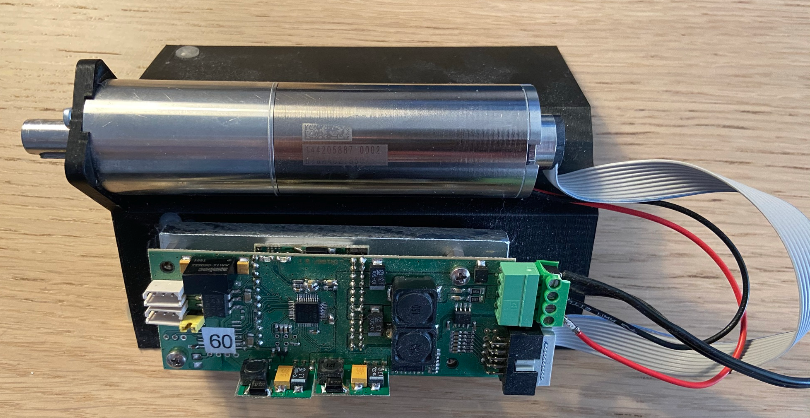
\includegraphics[angle=180,width=0.9\textwidth]{../Thesis/obrazky/dcmotor}
			\caption{DCMotor controller.}
			\label{fig:fliplink_orig}
		\end{minipage}\hfill
		\begin{minipage}[t]{0.45\textwidth}
			\centering
			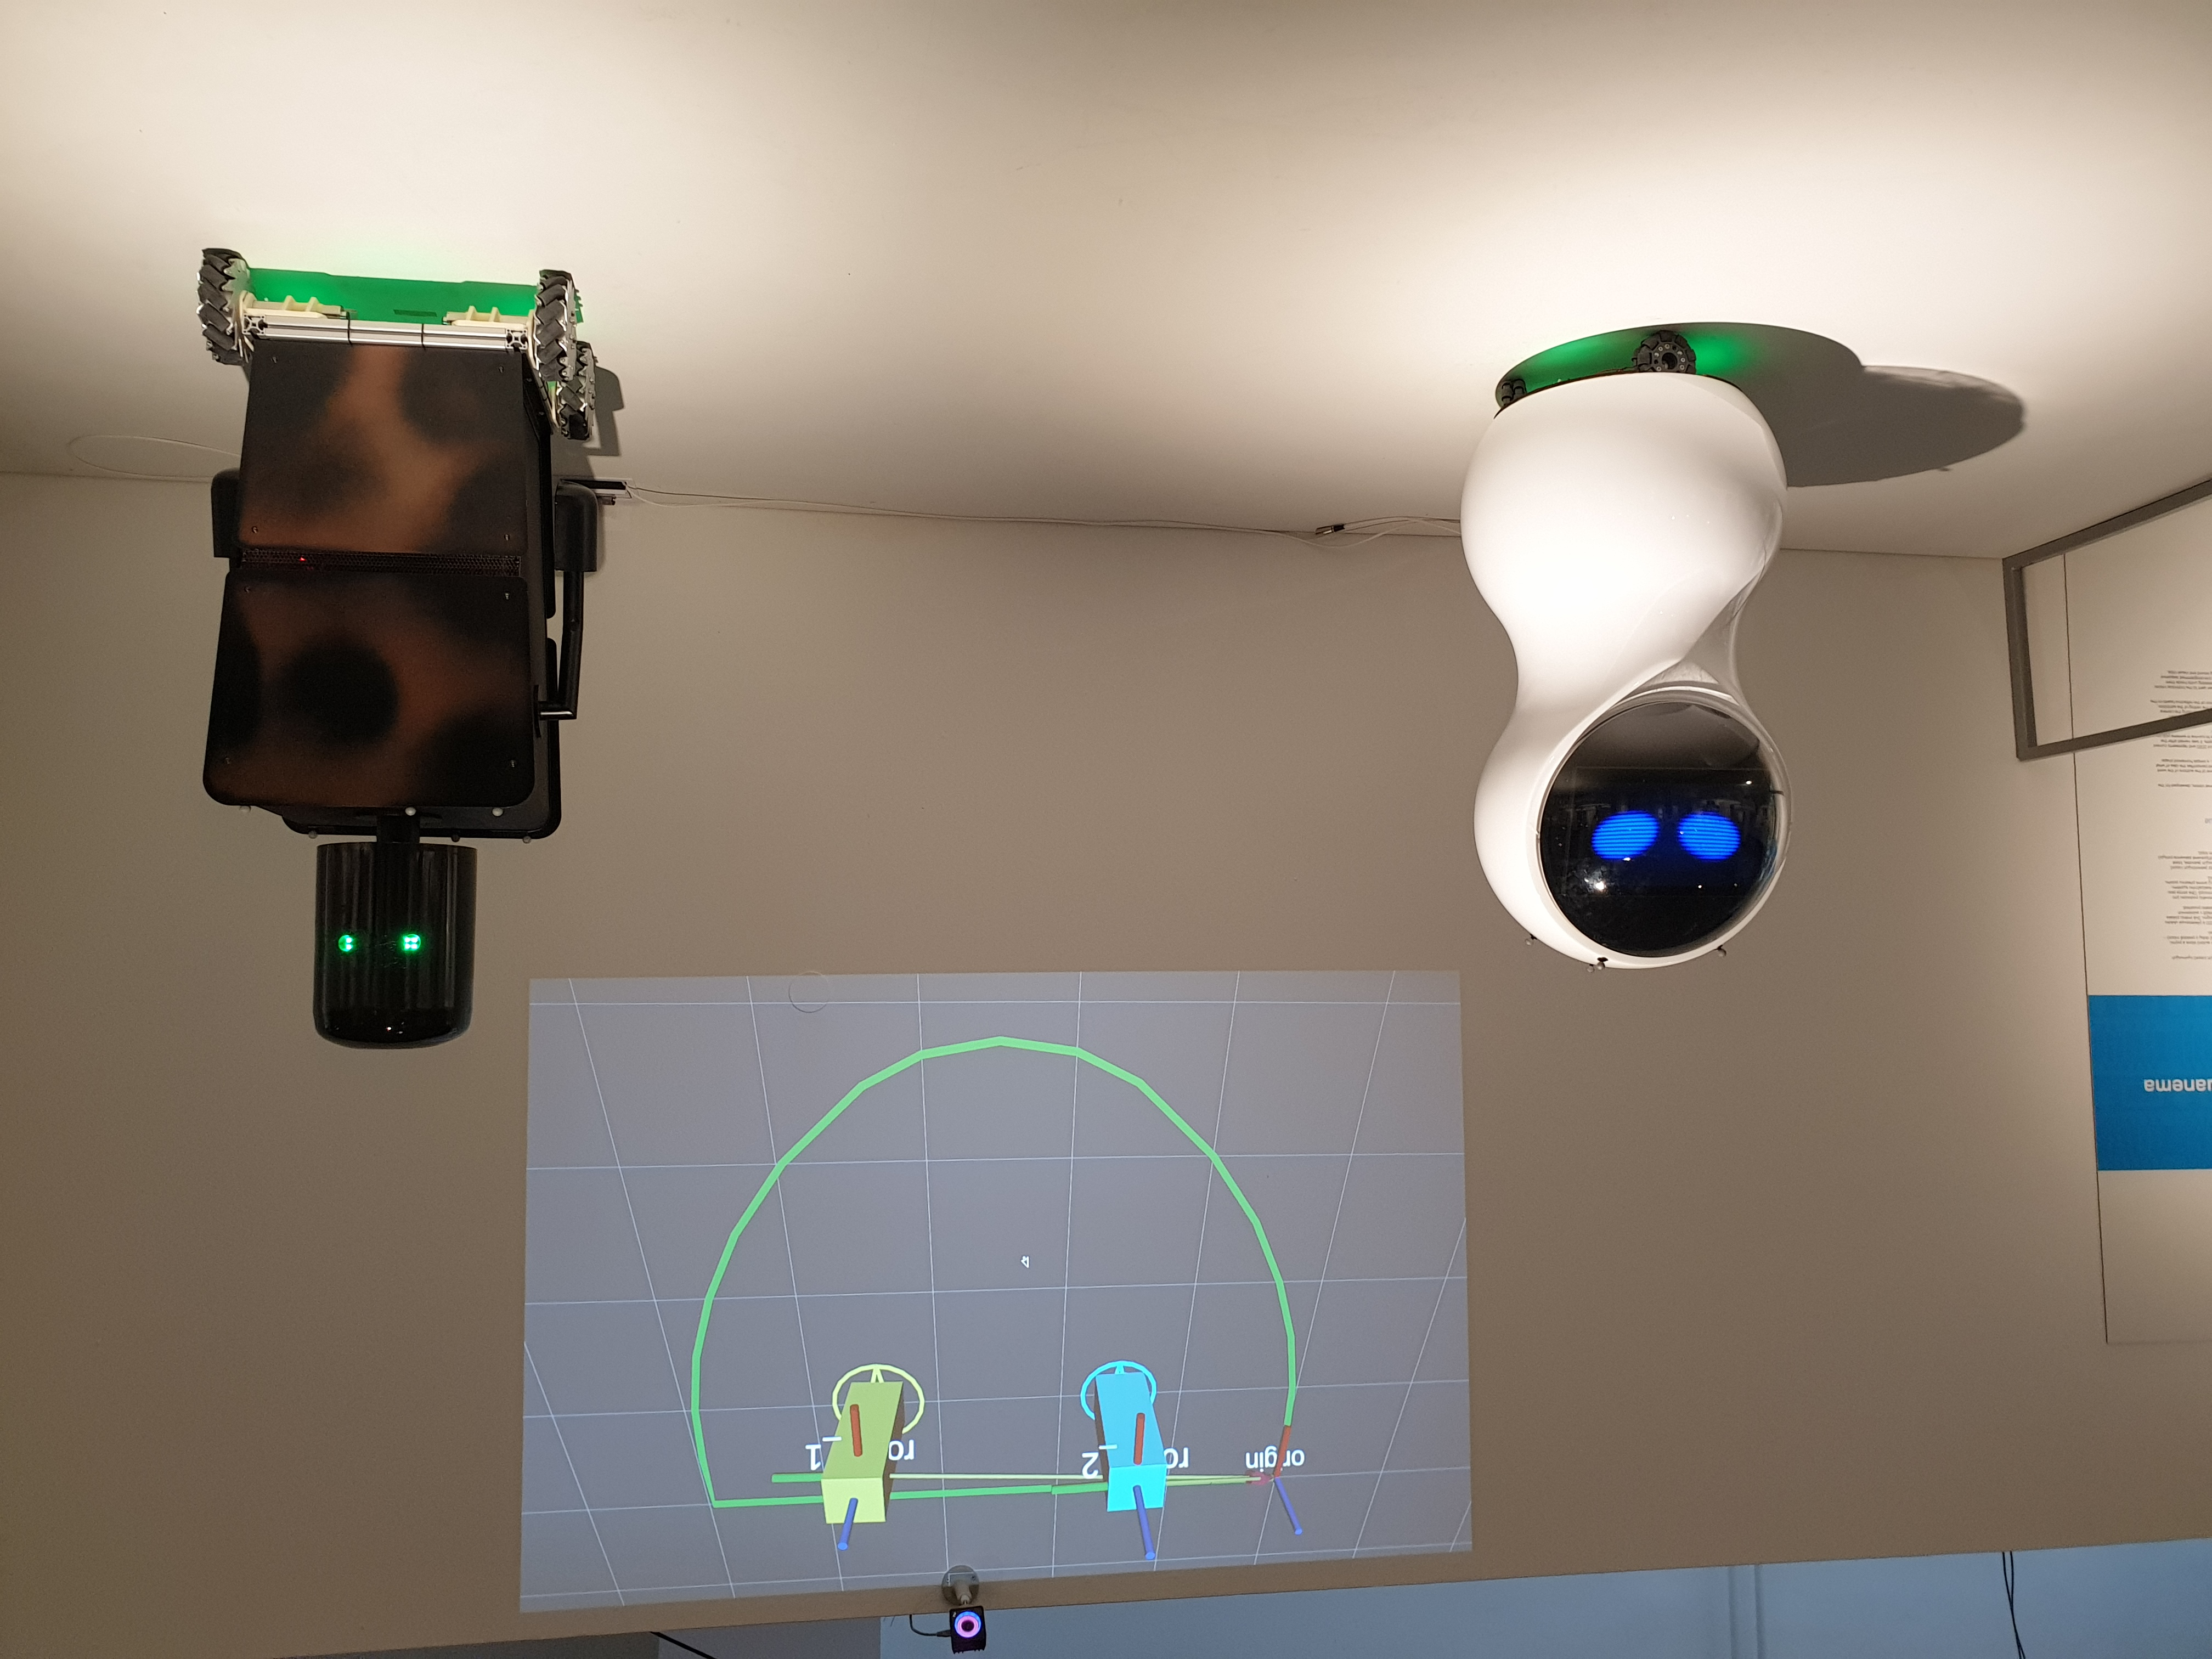
\includegraphics[angle=180,width=0.65\textwidth]{../Thesis/obrazky/karlozo_auanemozo}
			\caption{Roboti Karel a Auanema - 7 měničů s firmware v Rustu}
			\label{fig:fliplink_changed}
		\end{minipage}
	\end{figure}
\end{frame}
\begin{frame}
	% nadpis snímku
	\frametitle{Současné řešení}
	\begin{columns}[T] 								% prostředí sloupce s umístěním nahoře
		\begin{column}{0.5\textwidth}
			KM2
			\begin{itemize}
				\item ATMega8
				\item I\textsuperscript{2}C
				\item Napevno nastaveny proud
				\item Moduly s drivery do 3D tiskaren
			\end{itemize}
			\begin{figure}%
				\centering
				\vspace{0.2cm}	              % horizontální mezera
				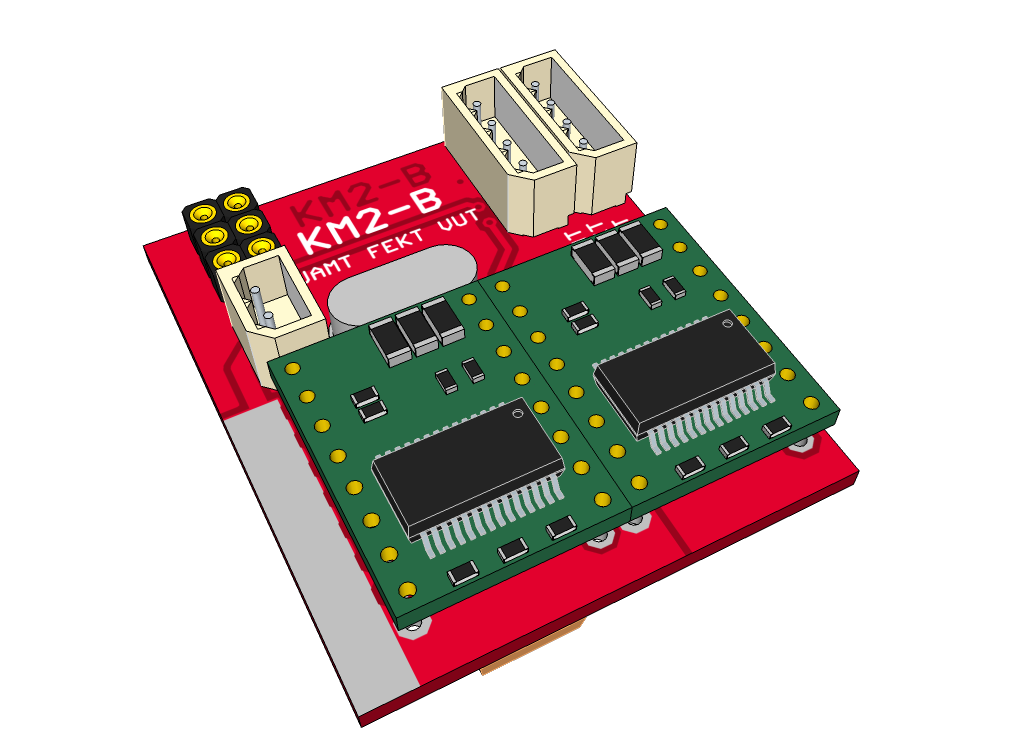
\includegraphics[width=0.5\columnwidth]{../Thesis/obrazky/km2render}
				\caption{Render kontroleru KM2}
				\label{fig:km2}
			\end{figure}
		\end{column}
		%
		\begin{column}{0.5\textwidth}
			KM3
				\begin{itemize}
					\item STM32F031 - 48 MHz, 32 kB FLASH, 4 kB RAM
					\item Integrovane drivery DRV8825
					\item Dynamicke nastavovani proudu
					\item Firmware v Rustu
				\end{itemize}
				\begin{figure}%
					\centering
					\vspace{0.1cm}	              % horizontální mezera
					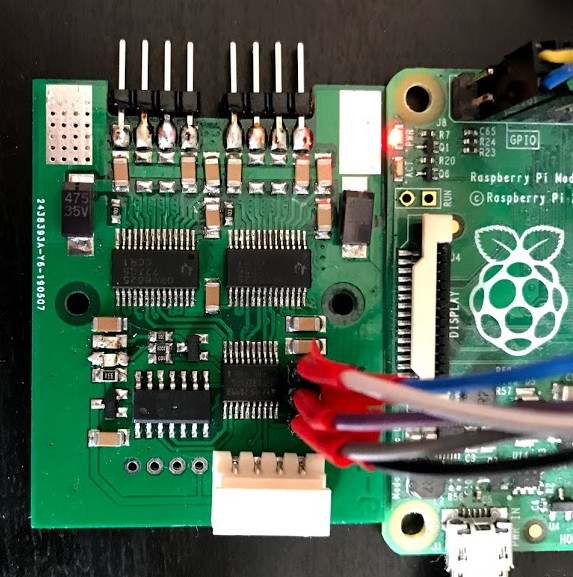
\includegraphics[width=0.4\columnwidth]{../Thesis/obrazky/km3}
					\caption{Kontroler KM2}
					\label{fig:km3}
				\end{figure}
		\end{column}
	\end{columns}											% ukončení prostředí
\end{frame}

\begin{frame}
	% nadpis snímku
	\frametitle{Požadavky}
	\begin{itemize}
		\item \textbf{FR-04} All relevant values (currents, timings, limits, etc.) shall be configurable via USB or CANOpen SDO protocol.
		\item \textbf{FR-06} The controller shall support control in speed mode as well as position mode.
		\item \textbf{FR-07} The controller shall provide basic electrical safety features - such as fuses and reverse voltage protection.
		\item \textbf{NFR-01} The controller shall provide developer-friendly protocol and data formats.
		\item \textbf{NFR-04} The firmware shall be easily extensible.
		\item \textbf{NFR-05} The firmware shall employ unit testing for QA (Quality Assurance).
		\item \textbf{C-01} The controller shall utilize stepper drivers with silent operation, such as Trinamic StealthChop\texttrademark.
		\item \textbf{C-03} The controller shall feature CAN bus, I2C bus and USB.
		\item \textbf{C-07} The firmware for the controller shall be developed using the Rust programming language.
	\end{itemize}
\end{frame}
\begin{frame}
	% nadpis snímku
	\frametitle{Technické řešení - vývoj elektroniky}
	\begin{columns}[T] 								% prostředí sloupce s umístěním nahoře
		\begin{column}{0.4\textwidth}
			\begin{itemize}
				\item Dvě revize
				\item STM32F405
				\item TMC2100/TMC2226
				\item Podpora pro enkodéry
				\item 4-vrstva DPS
				\item Návrh v KiCAD
			\end{itemize}
		\end{column}
		%
		\begin{column}{0.6\textwidth}		% druhý sloupec
			\begin{figure}%
				\centering              % horizontální mezera
				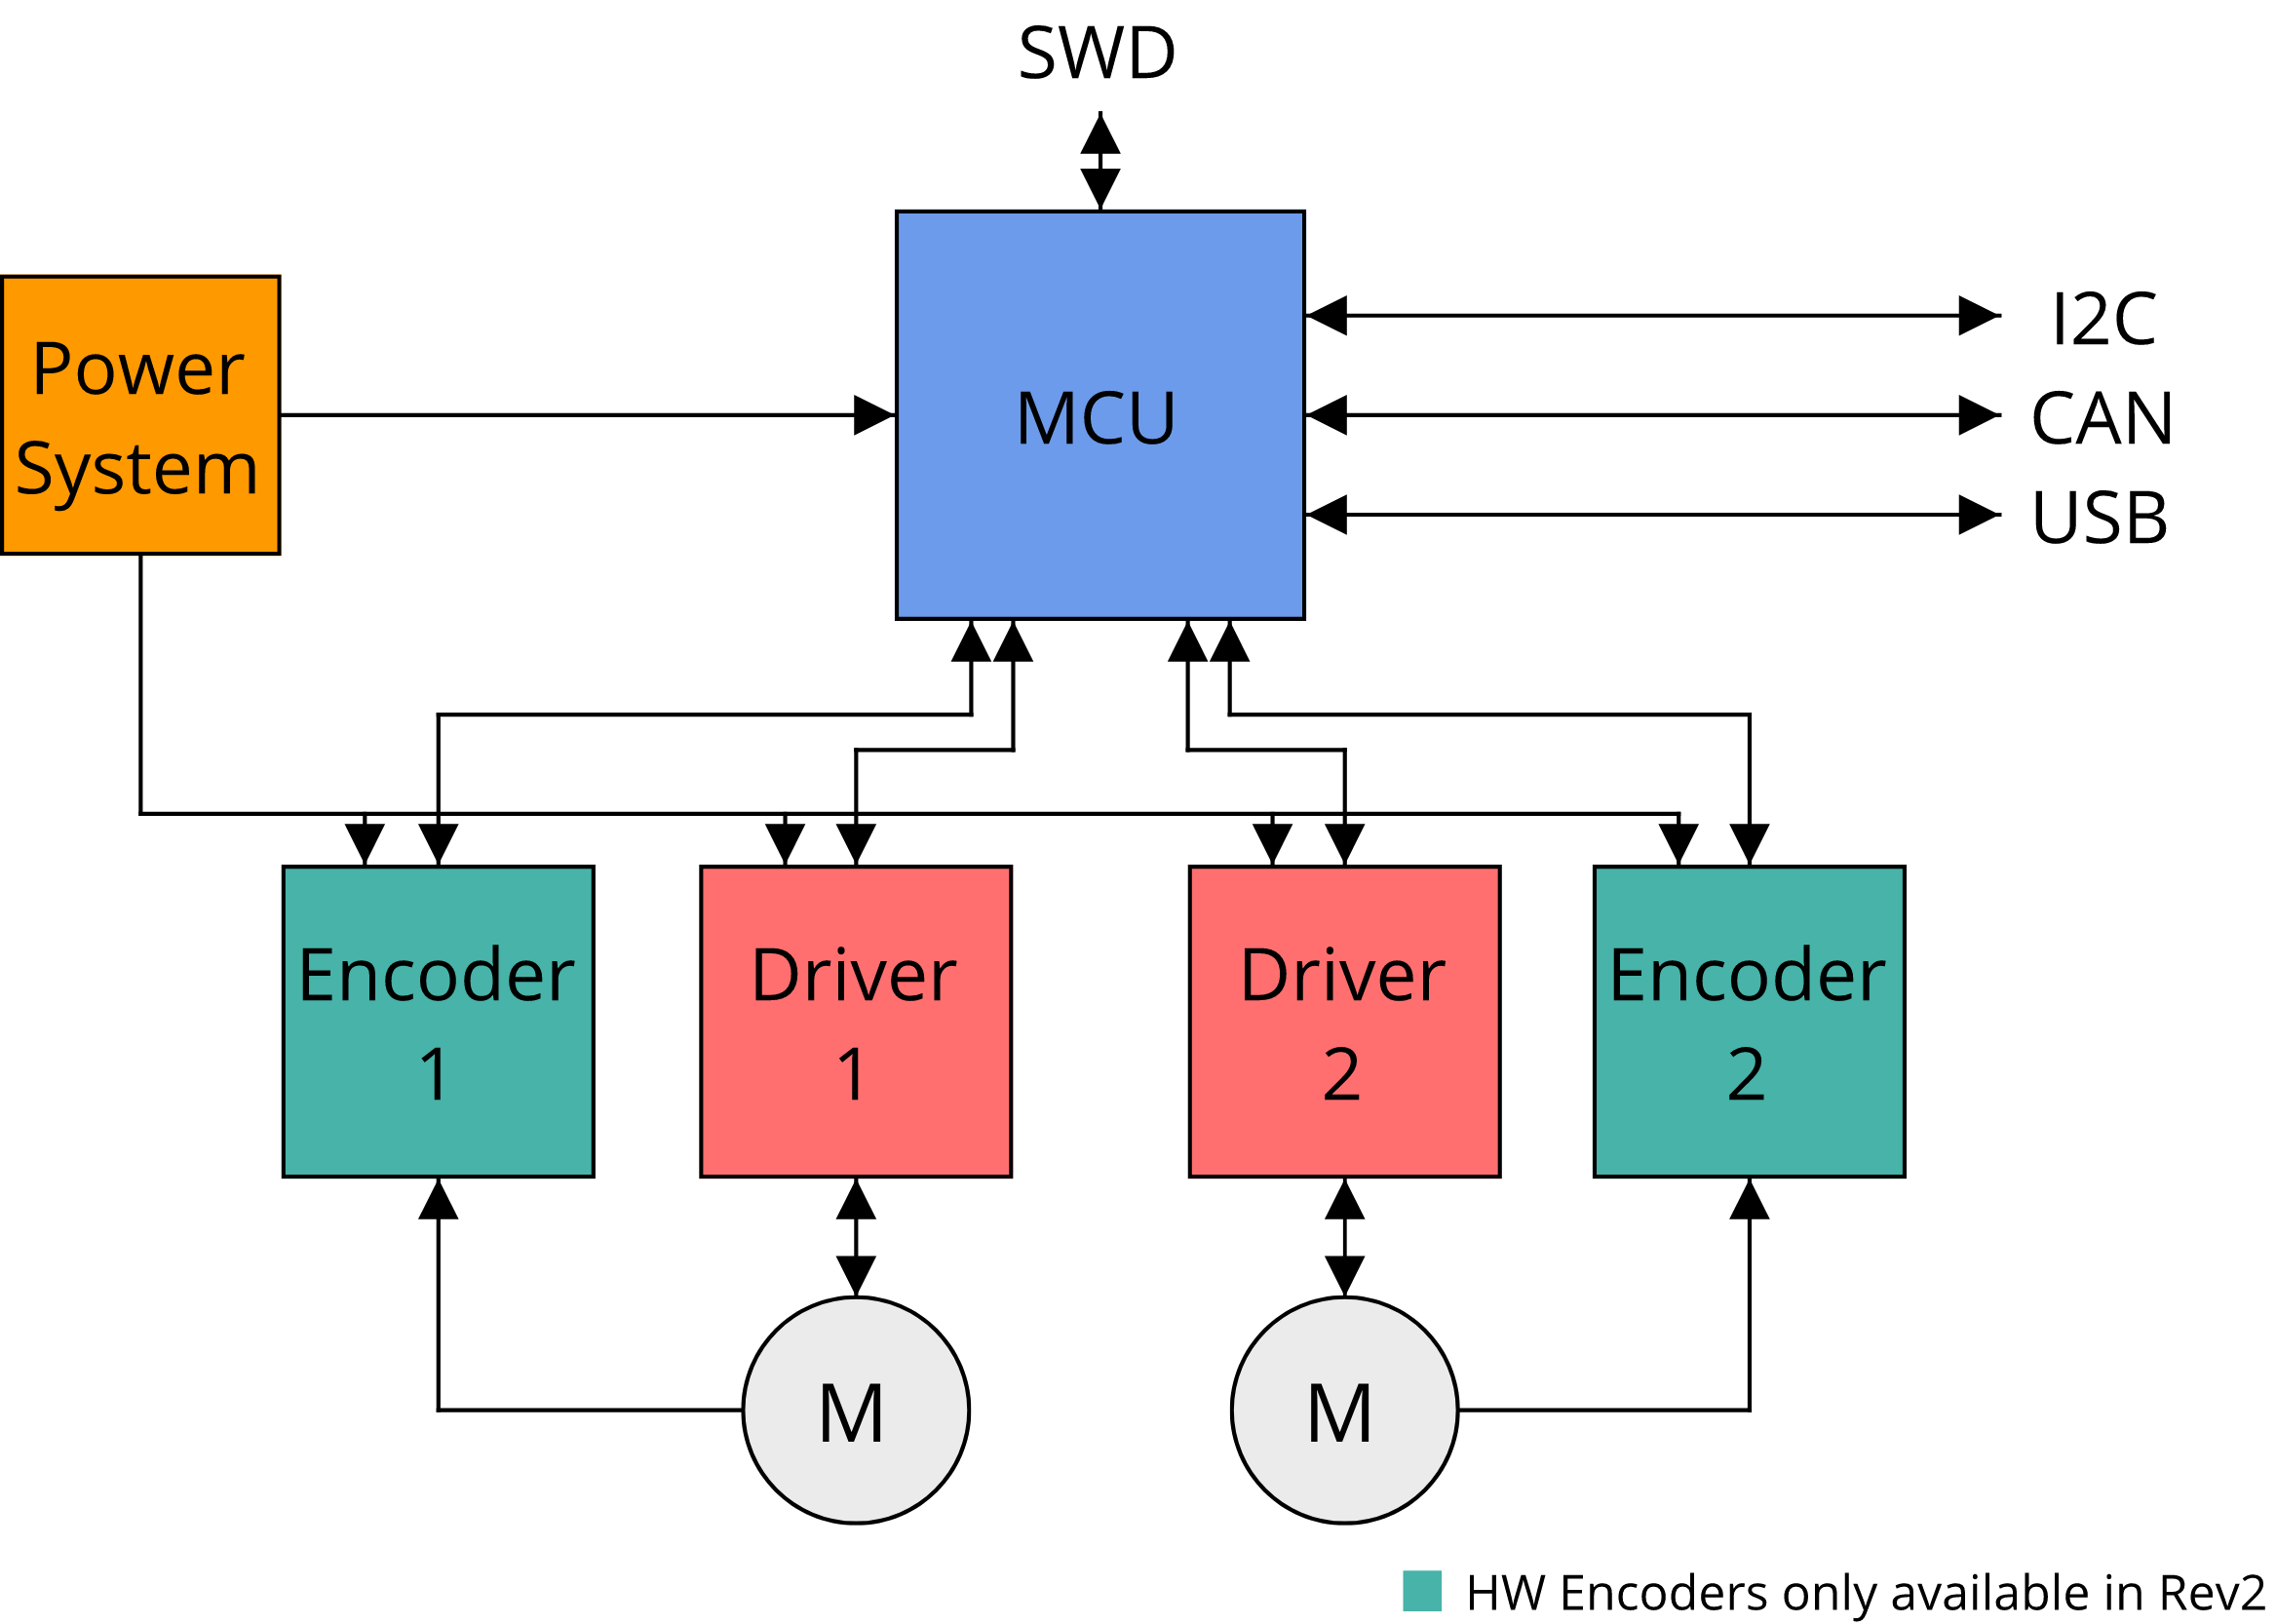
\includegraphics[width=0.8\columnwidth]{../Thesis/obrazky/sm4_block_diagram}
				%lze vložit popisek, ale povetšinou je to v prezentaci zbytečné
				\caption{Blokove schema menice}%
				\label{fig:sm4_block}
			\end{figure}
		\end{column}
	\end{columns}
\end{frame}
\begin{frame}
	% nadpis snímku
	\frametitle{Technické řešení - výsledná elektronika}
	\begin{columns}[T] 								% prostředí sloupce s umístěním nahoře
		\begin{column}{0.5\textwidth}		% první sloupec
			\begin{figure}%
				\centering	              % horizontální mezera
				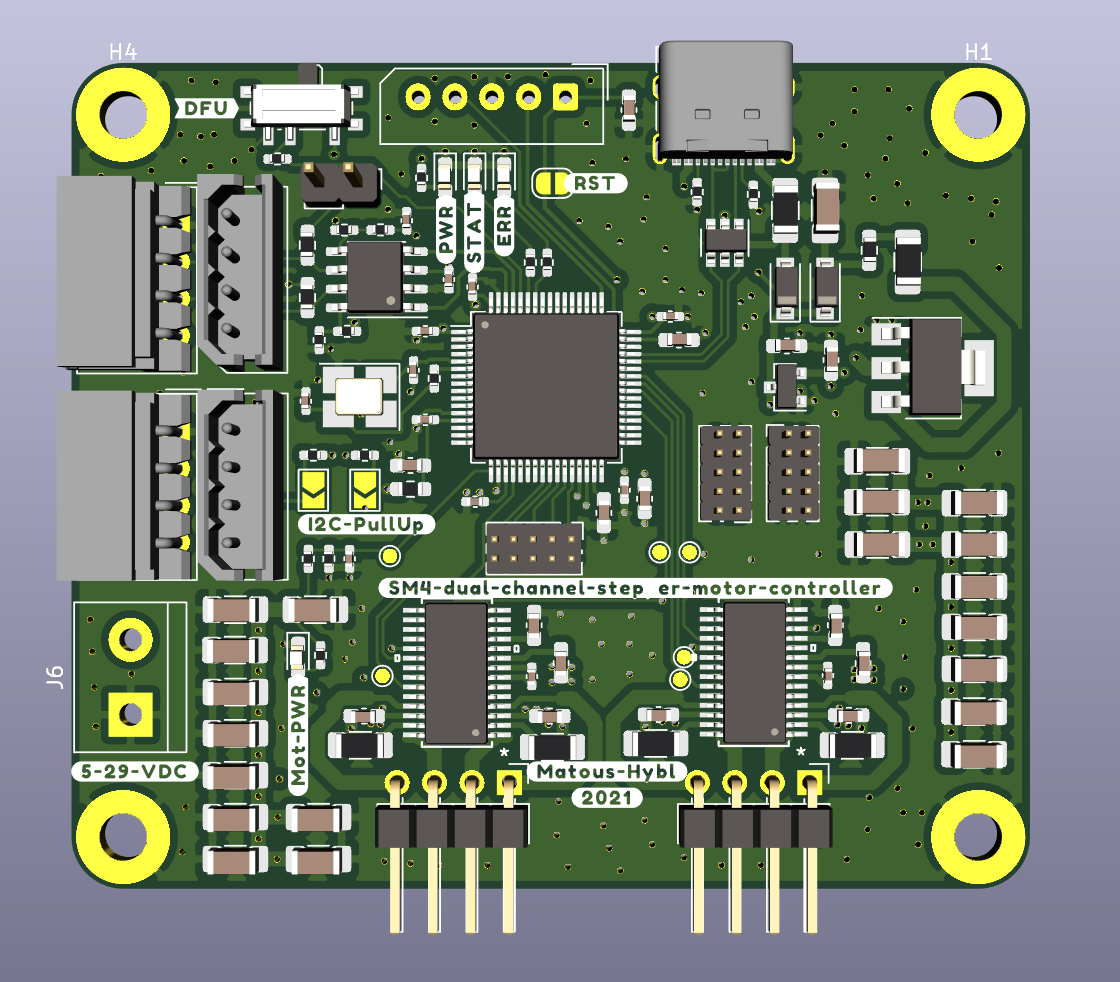
\includegraphics[width=0.8\columnwidth]{../Thesis/obrazky/pcb_rev2}
				%lze vložit popisek, ale povetšinou je to v prezentaci zbytečné
				\caption{Blokove schema menice}%
				\label{fig:sm4_block}
			\end{figure}
		\end{column}
		%
		\begin{column}{0.5\textwidth}		% druhý sloupec
			\begin{figure}%
				\centering
				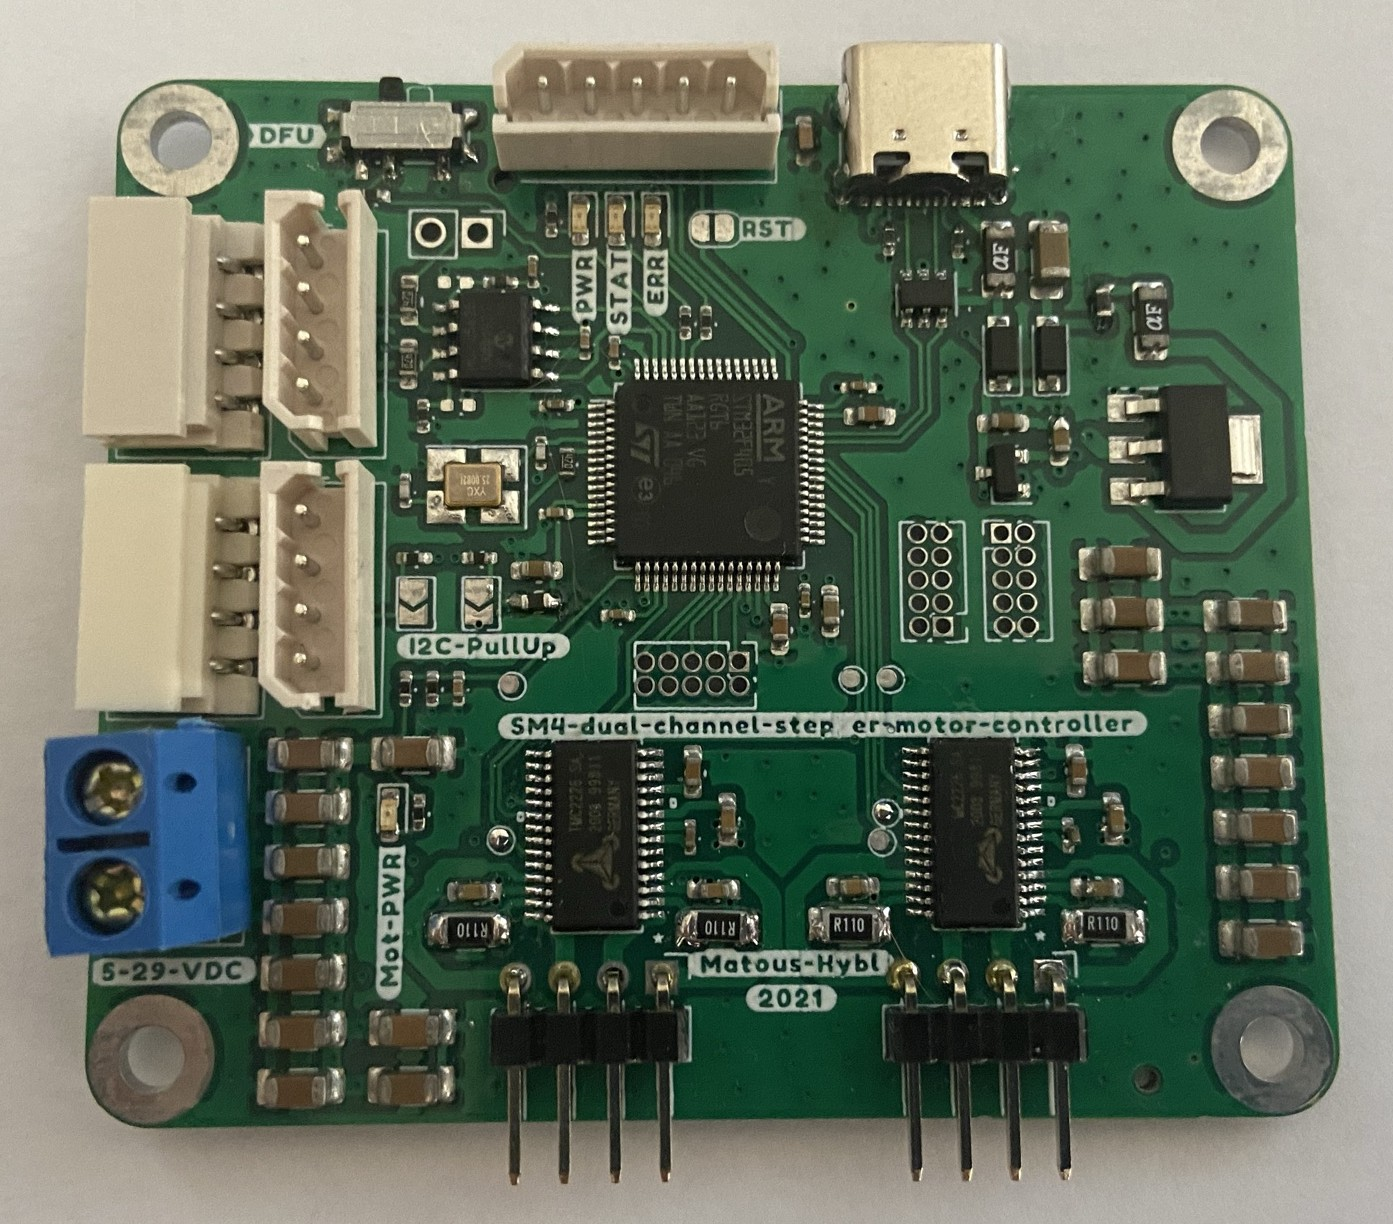
\includegraphics[width=0.8\columnwidth]{../Thesis/obrazky/rev2}
				%lze vložit popisek, ale povetšinou je to v prezentaci zbytečné
				\caption{Blokove schema menice}%
				\label{fig:sm4_block}
			\end{figure}
		\end{column}
	\end{columns}
\end{frame}
\begin{frame}
	% nadpis snímku
	\frametitle{Technické řešení - firmware}
	\begin{columns}[T] 								% prostředí sloupce s umístěním nahoře
		\begin{column}{0.5\textwidth}		% první sloupec
			\begin{itemize}
				\item Embedded Rust
				\item Založen na RTIC
				\item Využívá jak HAL, tak přímý přístup k HW
				\item Hojně využívá traits a generiku pro dependency injection
				\item Testovatelný (unit i integration testy)
			\end{itemize}
		\end{column}
		%
		\begin{column}{0.5\textwidth}		% druhý sloupec
			\begin{figure}%
				\centering
				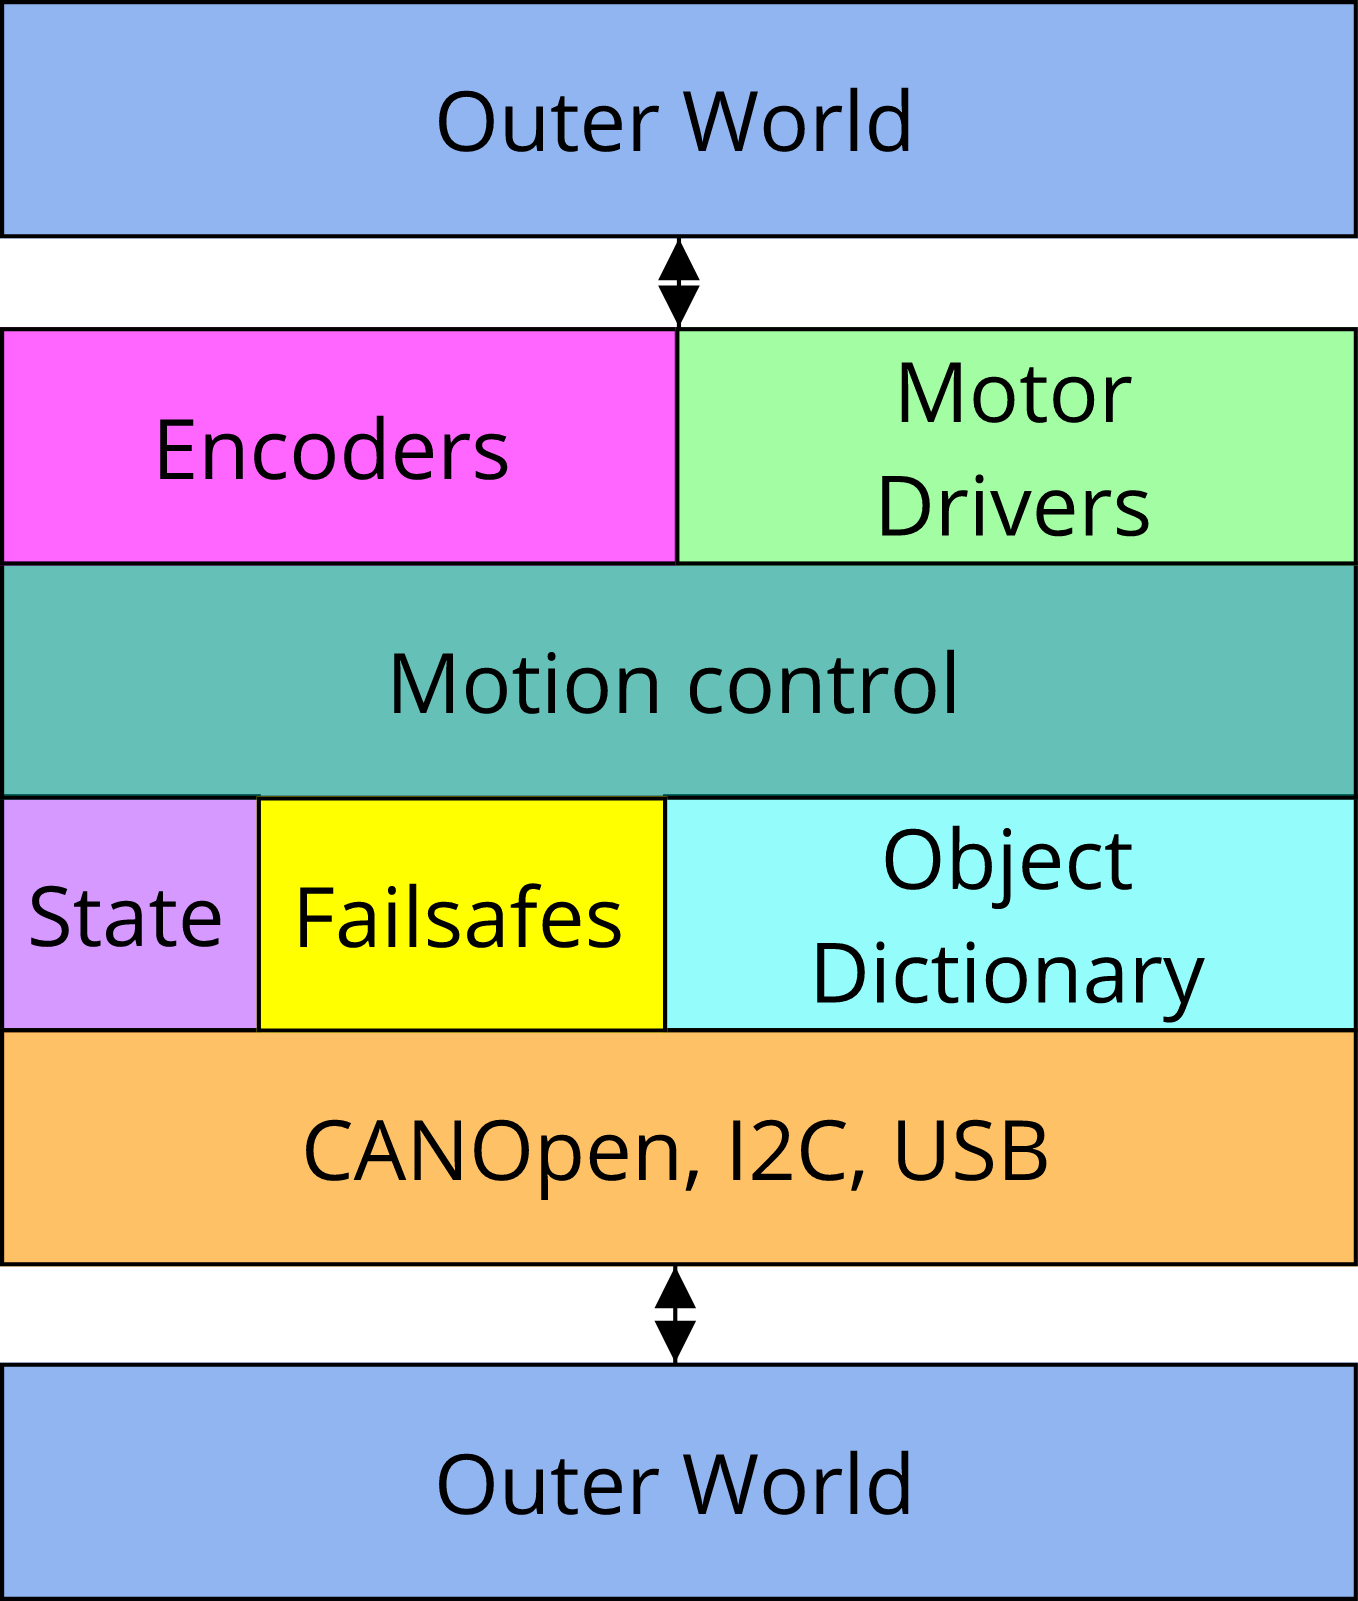
\includegraphics[width=0.7\columnwidth]{../Thesis/obrazky/firmware_arch}
				%lze vložit popisek, ale povetšinou je to v prezentaci zbytečné
				\caption{Blokove schema menice}%
				\label{fig:sm4_block}
			\end{figure}
		\end{column}
	\end{columns}
\end{frame}
\begin{frame}
	% nadpis snímku
	\frametitle{Technické řešení - Motion Control}
	\begin{figure}%
		\centering
		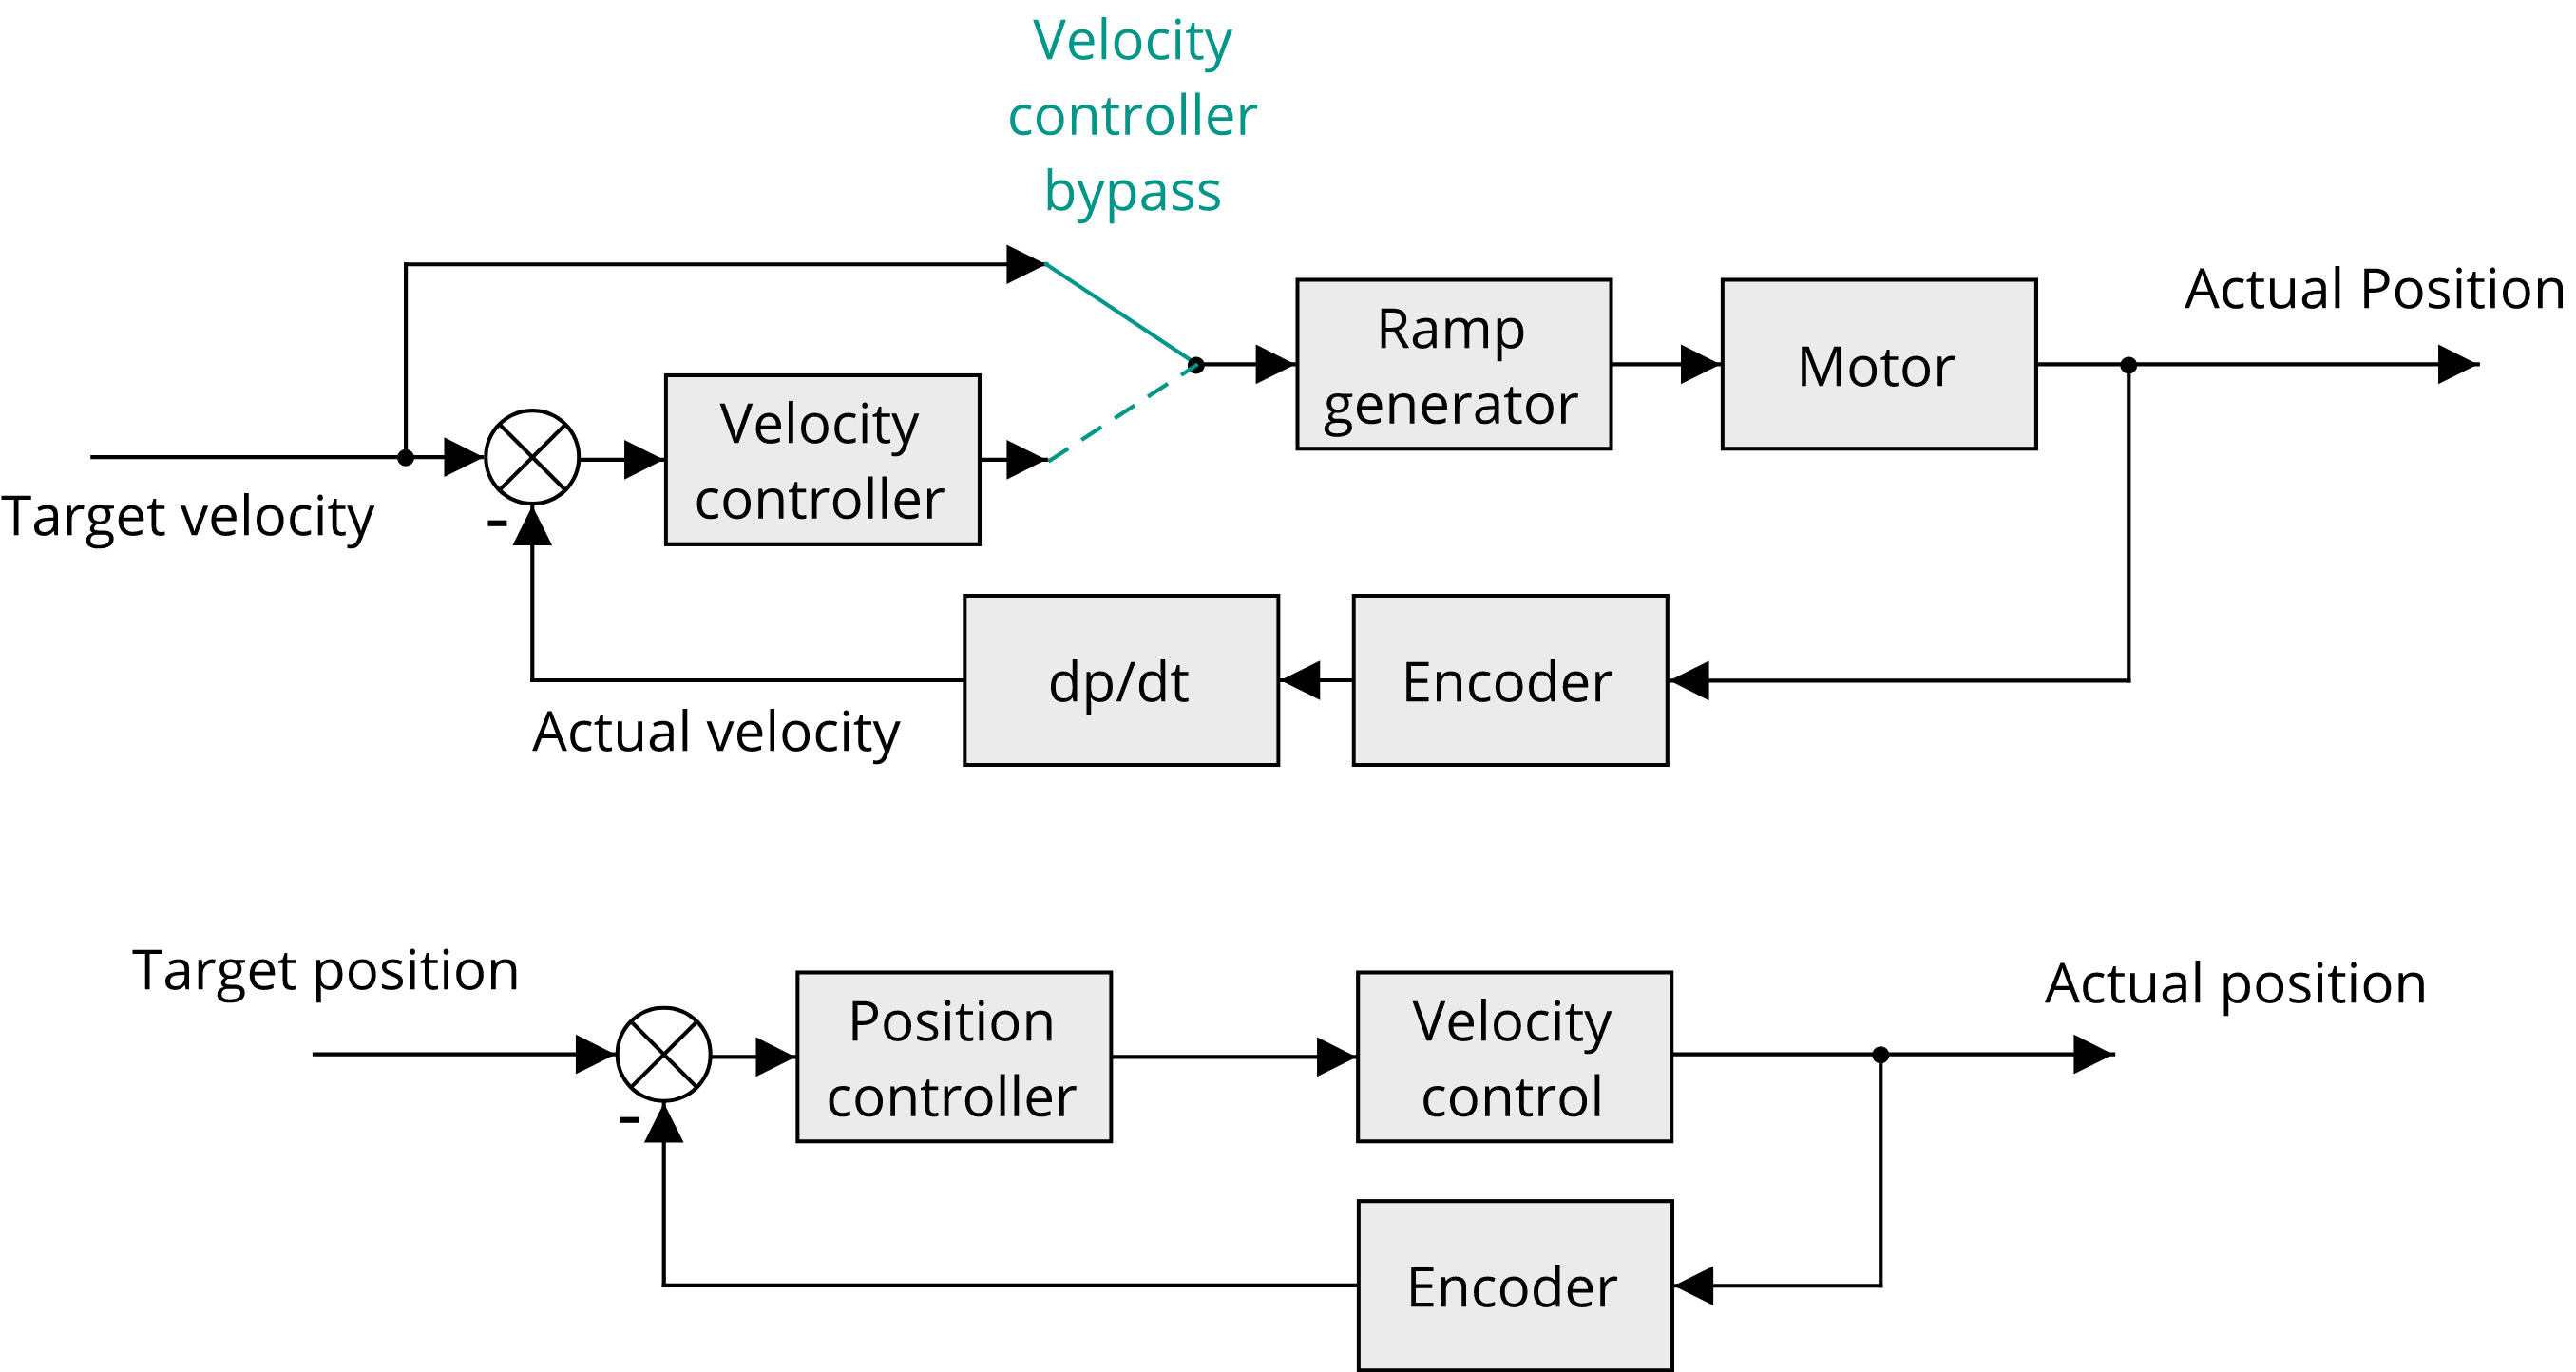
\includegraphics[width=0.8\textwidth]{../Thesis/obrazky/motion_control}
		%lze vložit popisek, ale povetšinou je to v prezentaci zbytečné
		\caption{Motion Control}%
		\label{fig:sm4_block}
	\end{figure}
\end{frame}
\begin{frame}
	% nadpis snímku
	\frametitle{Technické řešení - obslužný SW}
	\begin{columns}[T] 								% prostředí sloupce s umístěním nahoře
		\begin{column}{0.4\textwidth}
			\begin{itemize}
				\item TUI (Terminal User Interface)
				\item Komunikace přes CAN
				\item Možnost řízení obou os, v pozičním i rychlostním režimu
				\item V budoucnu GUI, možnost konfigurace parametrů
			\end{itemize}
		\end{column}
		%
		\begin{column}{0.6\textwidth}		% druhý sloupec
			\begin{figure}%
				\centering
				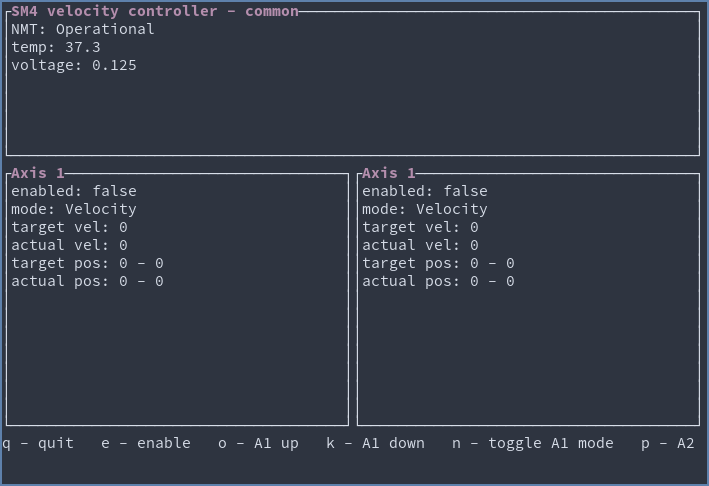
\includegraphics[width=0.8\columnwidth]{../Thesis/obrazky/tui}
				%lze vložit popisek, ale povetšinou je to v prezentaci zbytečné
				\caption{TUI ridici aplikace}%
				\label{fig:sm4_block}
			\end{figure}
		\end{column}
	\end{columns}
\end{frame}

\begin{frame}
	% nadpis snímku
	\frametitle{Demonstrace 1 - lineárni posuv}
	\begin{columns}[T] 								% prostředí sloupce s umístěním nahoře
		\begin{column}{0.4\textwidth}
			\begin{itemize}
				\item Jedna osa,
				\item poziční řízení,
				\item I\textsuperscript{2}C,
				\item pomocí druhé revize hardware bude možný sensorless homing.
			\end{itemize}
		\end{column}
		%
		\begin{column}{0.6\textwidth}		% druhý sloupec
			\begin{figure}%
				\centering
				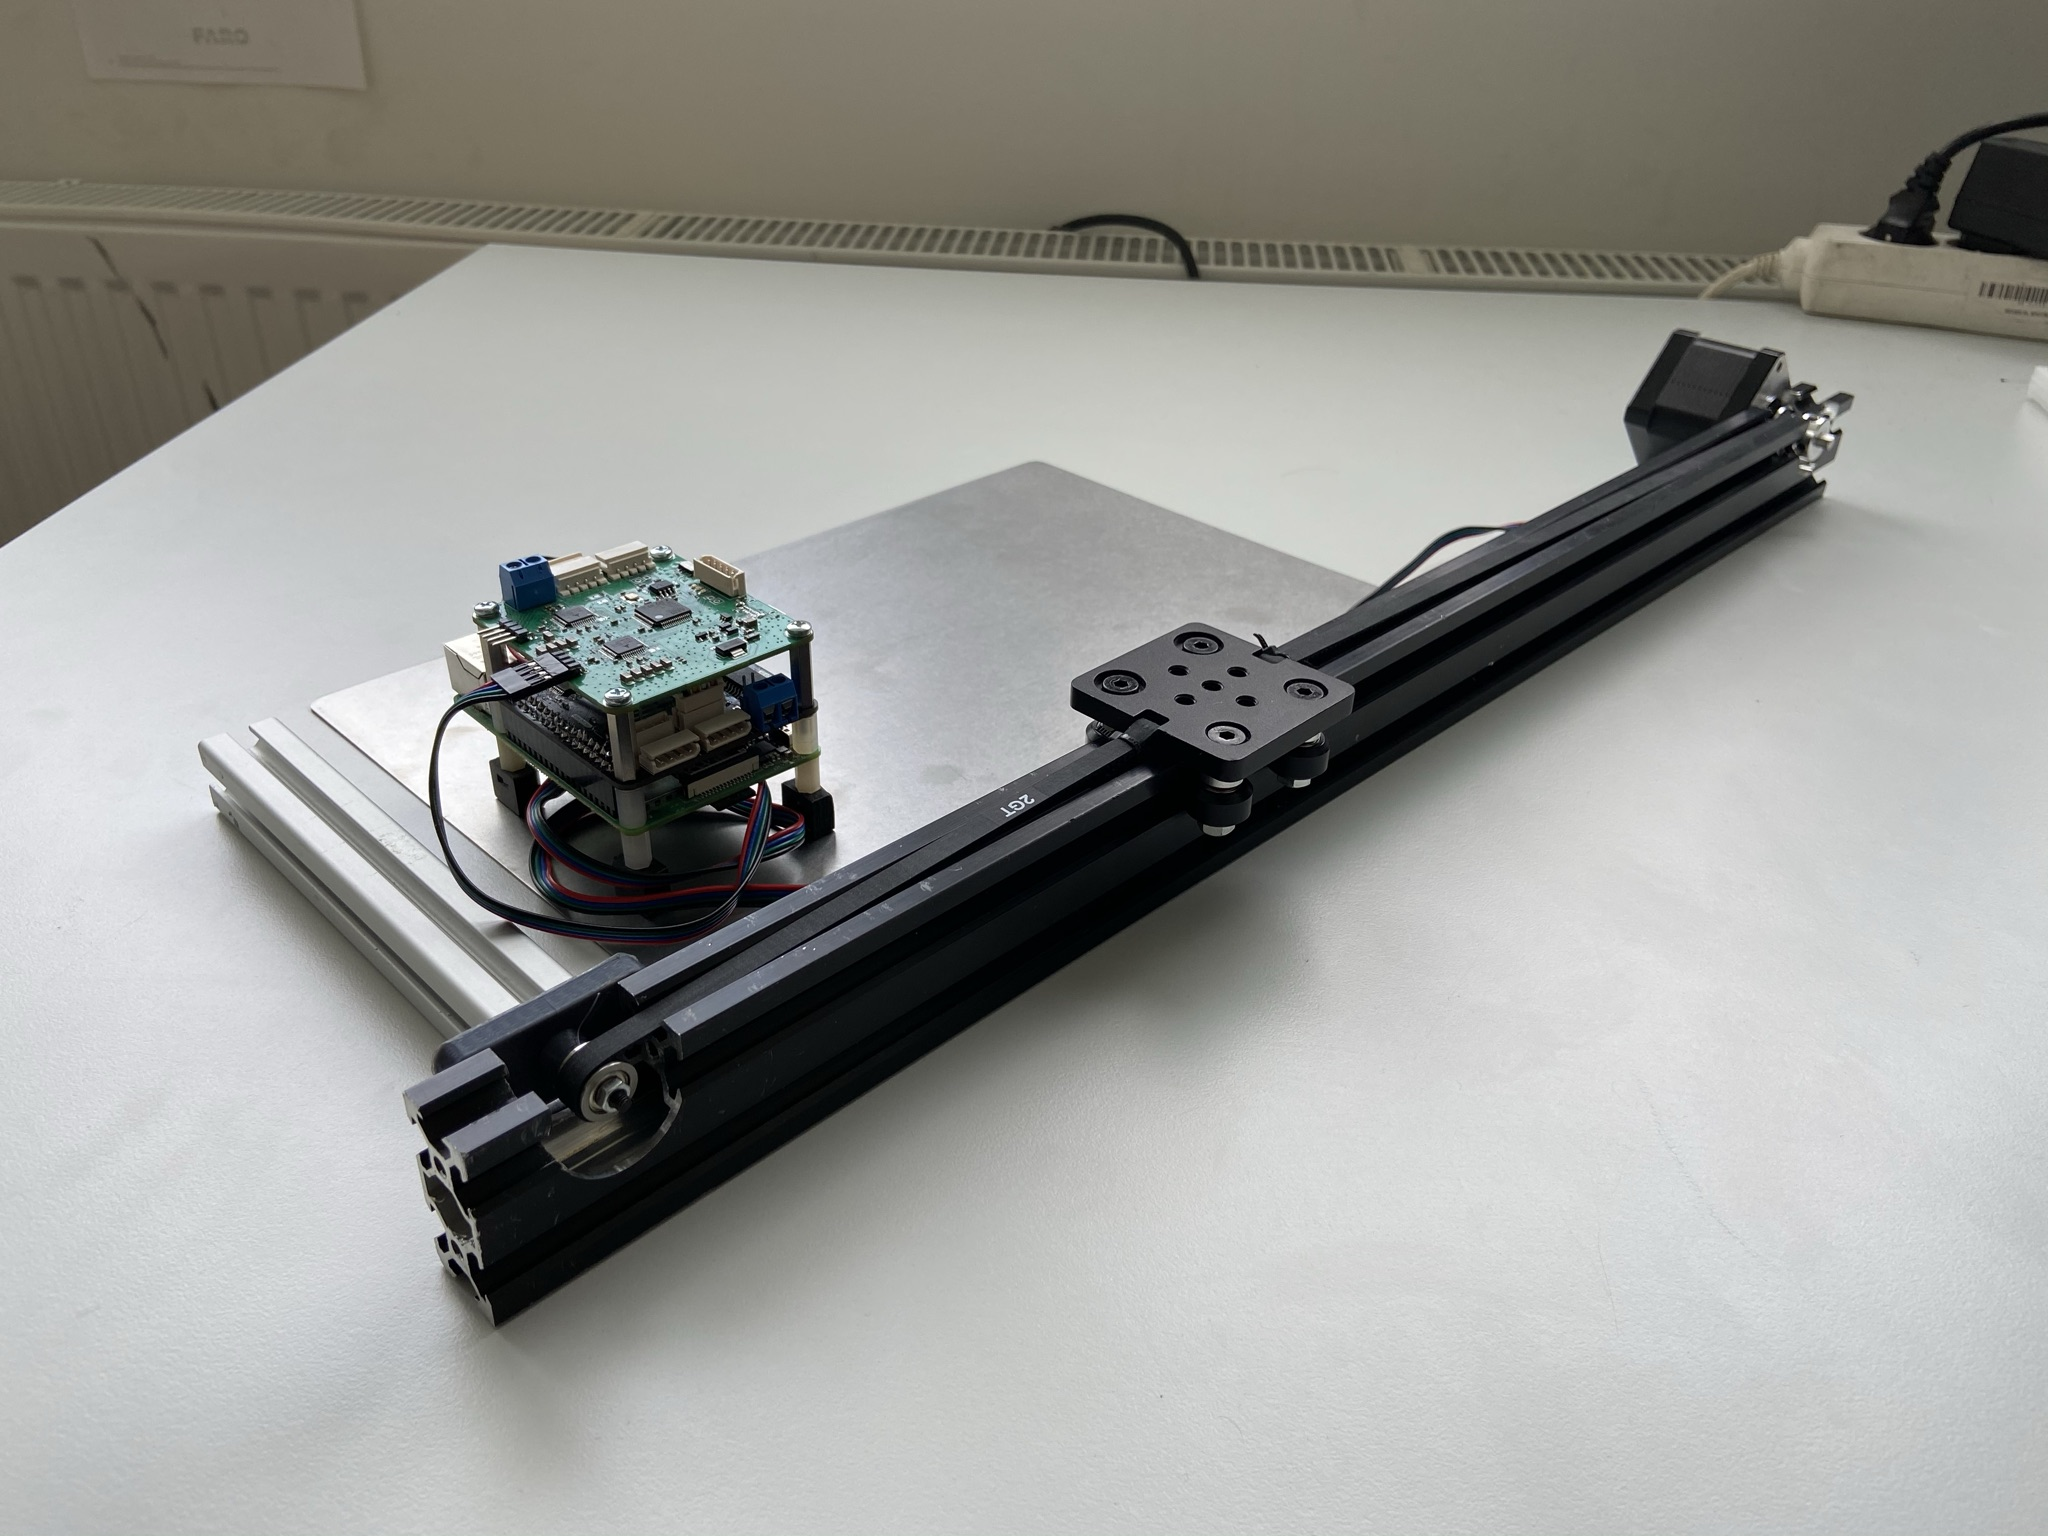
\includegraphics[width=0.8\columnwidth]{../Thesis/obrazky/rail}
				%lze vložit popisek, ale povetšinou je to v prezentaci zbytečné
				\caption{Lineární posuv}%
				\label{fig:sm4_block}
			\end{figure}
		\end{column}
	\end{columns}
\end{frame}

\begin{frame}
	% nadpis snímku
	\frametitle{Demonstrace 1 - lineární posuv}
	\movie[width=14cm,height=7cm,poster,autostart,repeat,showcontrols=true]{}{sample-mp4-file.mp4}
\end{frame}

\begin{frame}
	% nadpis snímku
	\frametitle{Demonstrace 2 - mapovací robot}
	\begin{columns}[T] 								% prostředí sloupce s umístěním nahoře
		\begin{column}{0.4\textwidth}
			\begin{itemize}
				\item Obě osy,
				\item rychlostní řízení,
				\item CAN bus,
				\item do budoucna pomůcka do předmětu MPC-MAP.
			\end{itemize}
		\end{column}
		%
		\begin{column}{0.6\textwidth}		% druhý sloupec
			\begin{figure}%
				\centering
				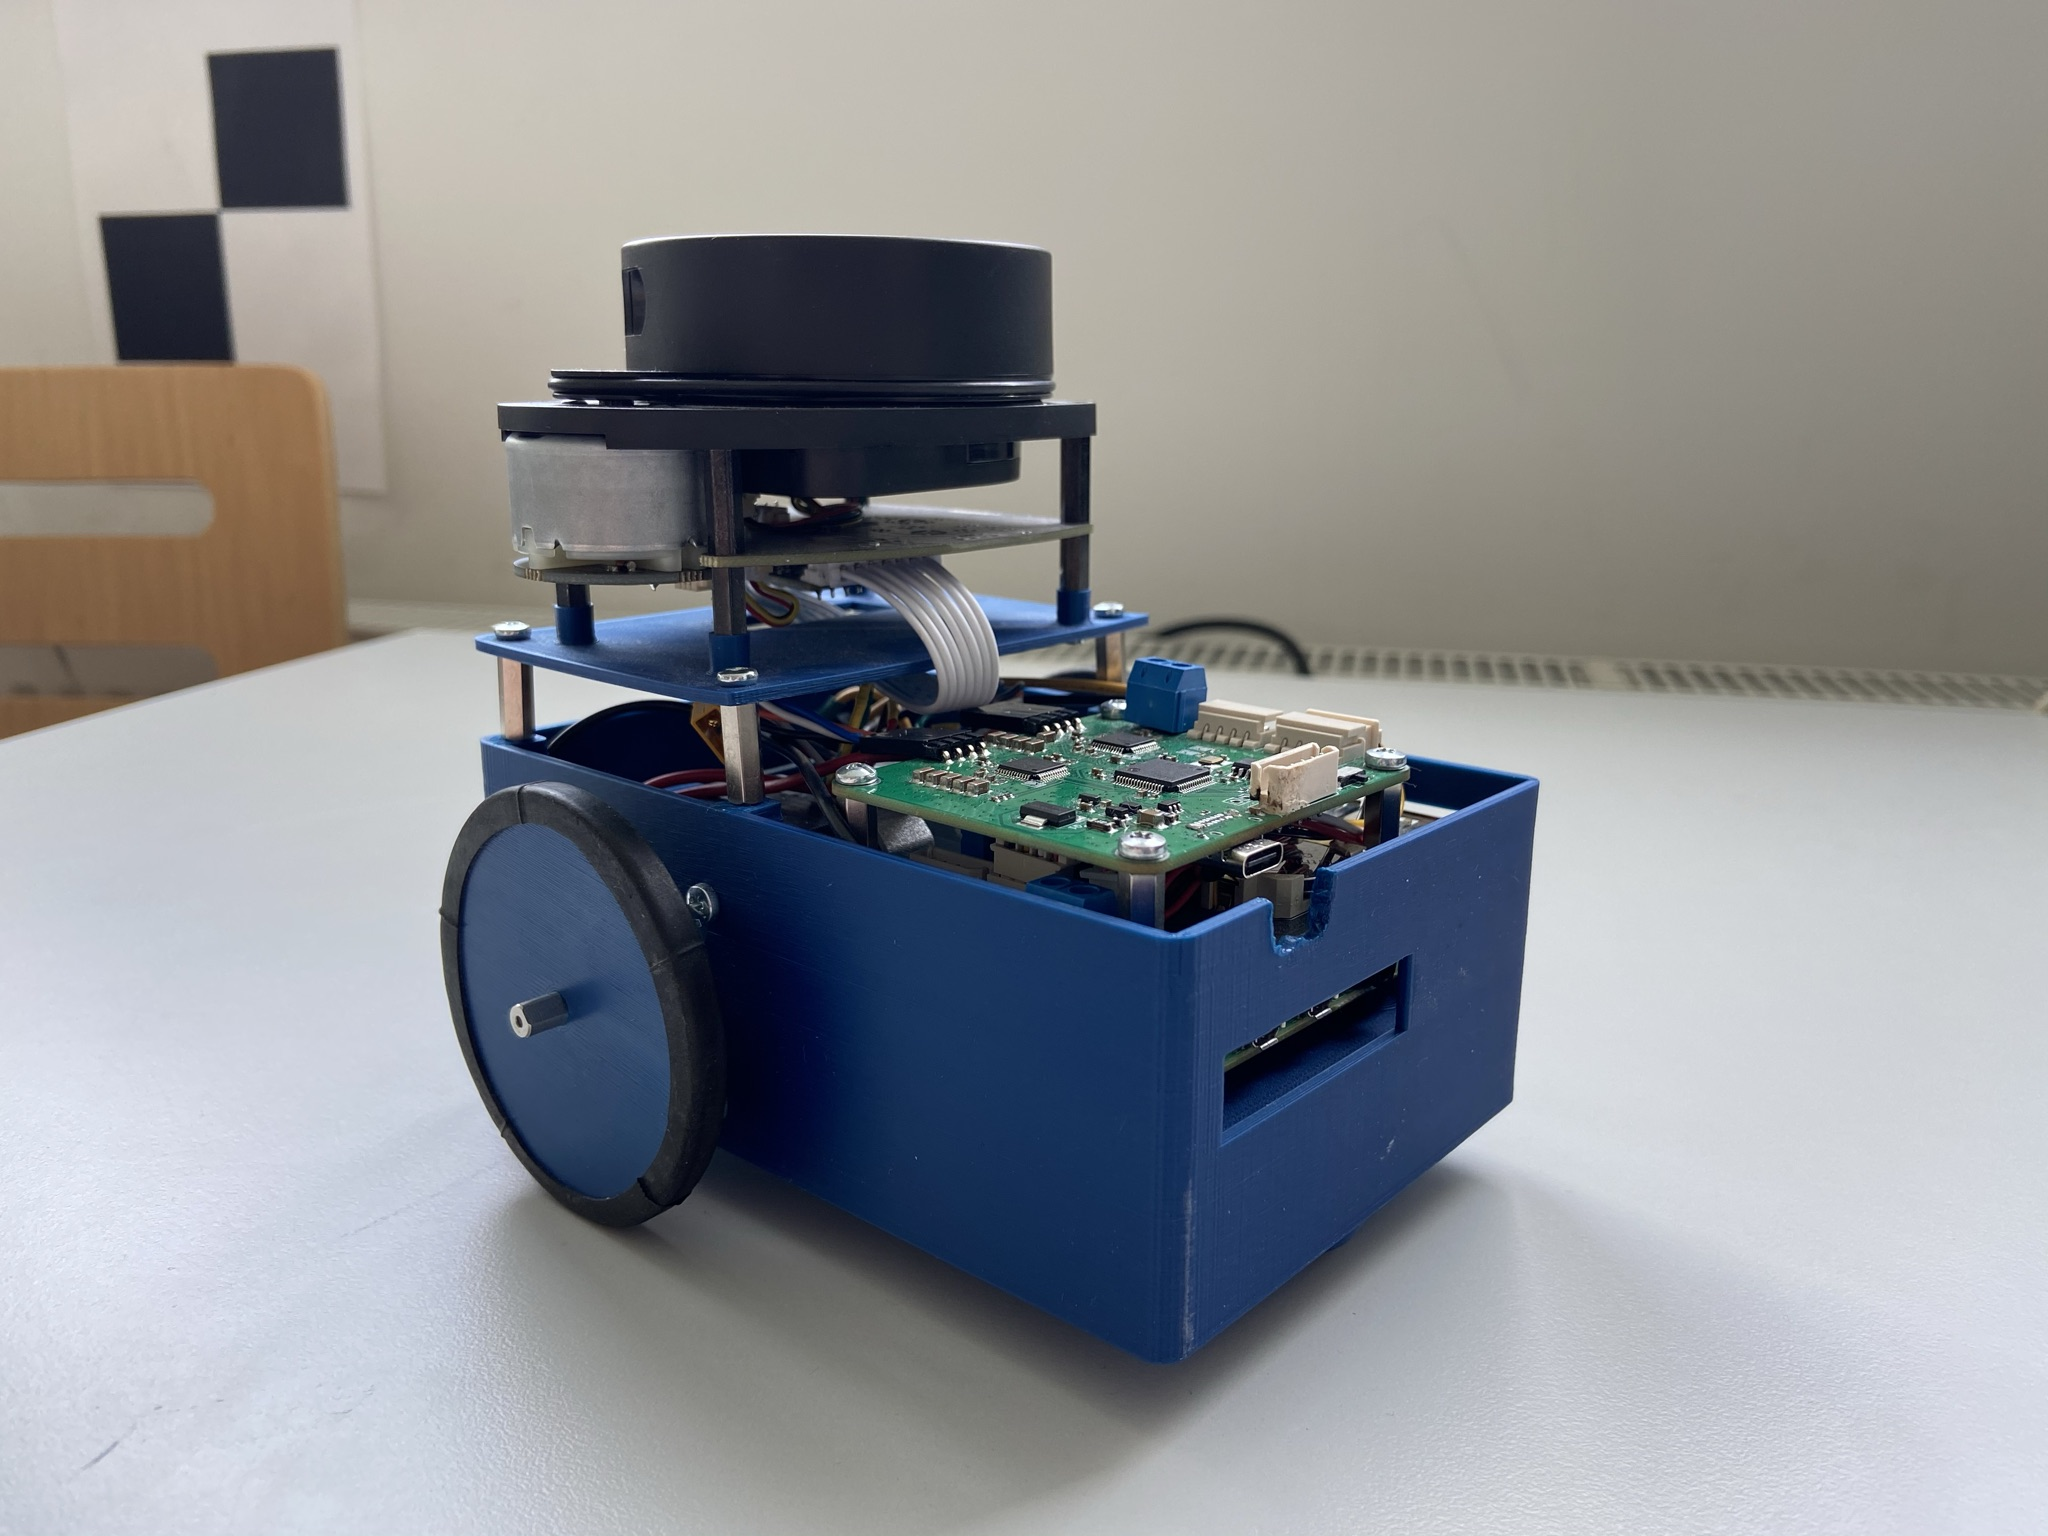
\includegraphics[width=0.8\columnwidth]{../Thesis/obrazky/map_bot}
				%lze vložit popisek, ale povetšinou je to v prezentaci zbytečné
				\caption{Mapovací robot}%
				\label{fig:sm4_block}
			\end{figure}
		\end{column}
	\end{columns}
\end{frame}

\begin{frame}
	% nadpis snímku
	\frametitle{Demonstrace 2 - mapovací robot}
	\movie[width=14cm,height=7cm,poster,autostart,repeat,showcontrols=true]{}{sample_640x360.avi}
\end{frame}

\begin{frame}
	% nadpis snímku
	\frametitle{Zhodnocení}
	\begin{itemize}
		\item Požadavky splněny až na výjimky, zadání splněno.
		\item Lze řídit obě osy, v obou režimech, pomocí obou komunikačních rozhraní.
		\item Embedded Rust se osvědčil i v tomto projektu.
	\end{itemize}
\end{frame}

\begin{frame}
	% nadpis snímku
	\frametitle{Budoucnost}
	\begin{itemize}
		\item GUI řídicí aplikace.
		\item Lepší podpora konfigurace měniče.
		\item Větší test coverage, integrační testy běžící v rámci CI.
		\item Doprogramování plné podpory druhé revize DPS.
	\end{itemize}
\end{frame}

%%%%%%%%%%%%%%
%\begin{frame}
%	\frametitle{Klíčové nástroje}
%
%	% prostředí 'alertblock', které slouží pro zdůraznění informace
%	\begin{alertblock}{Pro práci je klíčový Eulerův vzorec}
%		$$\eul^{\jmag x}=\cos x + \jmag\sin x$$
%	\end{alertblock}
%
%	\vspace{4ex}
%	Eulerova identita je speciálním případem tohoto vzorce, jestliže dosadíme $x=\uppi$\,:
%
%	% prostředí 'block', které slouží jako informativní
%	\begin{block}{Eulerova identita}
%		$$\eul^{\jmag \uppi}=\cos \uppi + \jmag\sin \uppi,$$\\
%		odkud vyplývá
%		$$\eul^{\jmag \uppi}+1=0.$$
%	\end{block}
%\end{frame}
%
%
%%%%%%%%%%%%%%
%\begin{frame}
%	\frametitle{Plošný spoj}
%
%	\begin{columns}[T] 								% prostředí sloupce s umístěním nahoře
%		\begin{column}{0.4\textwidth}		% první sloupec
%			Obrázek znázorňuje model:\\[2ex]
%			%
%			\begin{itemize}
%				\item Deska
%				\item Součástky
%				\item Signály
%				\item Napájení
%			\end{itemize}
%		\end{column}
%		%
%		\begin{column}{0.6\textwidth}		% druhý sloupec
%			\begin{figure}%
%				\centering
%				\vspace{1cm}	              % horizontální mezera
%				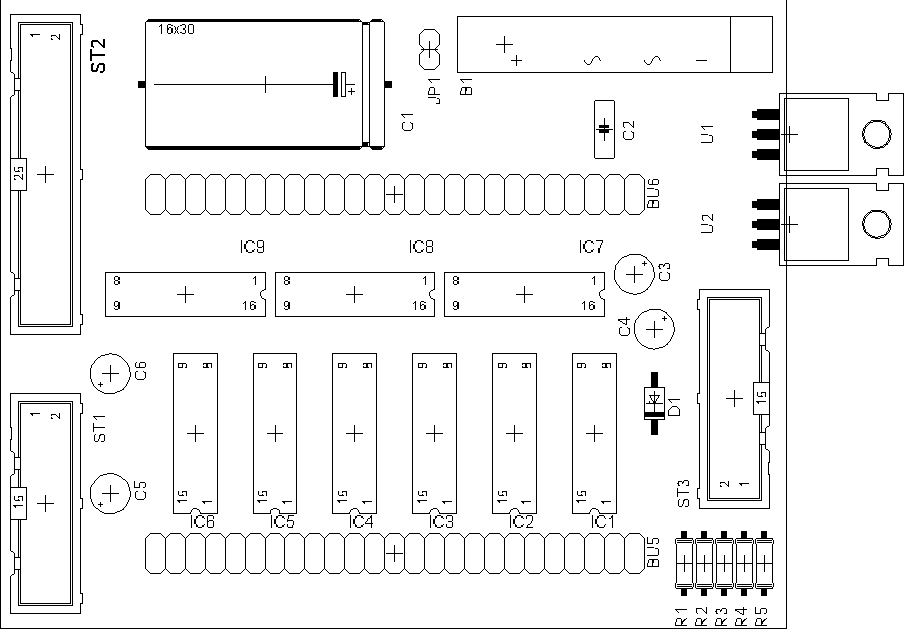
\includegraphics[width=0.8\columnwidth]{obrazky/soucastky}
%				%lze vložit popisek, ale povetšinou je to v prezentaci zbytečné
%				%\caption{Popisek obrázku}%
%				%\label{obr:ukazka}
%			\end{figure}
%		\end{column}
%	\end{columns}											% ukončení prostředí sloupce
%\end{frame}
%
%
%%%%%%%%%%%%%%
%\begin{frame}
%	\frametitle{Výsledky}
%	\vspace{1cm}
%	\begin{table}[]
%		\centering
%		\caption{Výsledky měření mobilních sítí}
%		\label{tab:tabulka}
%			\begin{tabular}{lcc}
%				\toprule
%					Technologie  & Rychlost stahování [kB/s] & Rychlost nahrávání [kB/s] \\
%				\midrule
%					GPRS (2,5G)	& 7,2 	& 3,6\\
%					UMTS 3G     & 48 		& 48\\
%					HSPA (3,5G)	&	1\,706	&	720\\
%					LTE (4G) 		& 40\,750 & 10\,750\\
%				\bottomrule
%			\end{tabular}
%	\end{table}
%\end{frame}
%
%
%%%%%%%%%%%%%%
%\begin{frame}
%	\frametitle{Závěr}
%	\dots
%\end{frame}


% podekovani
\begin{frame}[c] 
% bez nadpisu snímku
	\frametitle{\mbox{ }}
	\begin{center}
		{\Huge Děkuji za pozornost!}
	\end{center}
\end{frame}

% otázky oponenta
\frame{
\frametitle{Otázky oponenta}
	\emph{Jaká je souvislost Vašeho vzorce (1.2) s~Maxwellovými rovnicemi v~integrálním tvaru?}\\[2ex]
	%
	Již staří Římané\,\dots
}

\end{document}
